Die Nacht war kurz, denn wir mussten früh raus, um zeitig über die Golden Gate Bridge zu fahren zu unserem Ziel Pier~39.
Von dort laufen die Fähren nach Alcatraz aus.
Einem Betonklumpen in der Bucht von San Francisco.
Aber wenn die Amerikaner etwas können, dann ist es Unterhaltung.
Der Audio-Guide

\begin{tikzpicture}[remember picture, overlay]
\node[inner sep=0pt, yshift=-.2\paperheight] at (current page.north) {%
	\includegraphics[width=\paperwidth,height=.45\paperheight]{20/hostel_marin_headlands_kleiner.jpg};%
};
%\node[inner sep=0pt, yshift=.25\paperheight] at (current page.south) {%
%	\includegraphics[width=\paperwidth,height=.5\paperheight]{21/image20160420_193101911.jpg};%
%};
\end{tikzpicture}

\vspace*{.27\paperheight}

\noindent
Audio-Guide hauchte dem Klumpen richtig Leben ein und so wurde eine empfehlenswerte Attraktion daraus.

\thispagestyle{empty}
\begin{tikzpicture}[remember picture, overlay]
\node[inner sep=0pt, yshift=.25\paperheight] at (current page.south) {%
	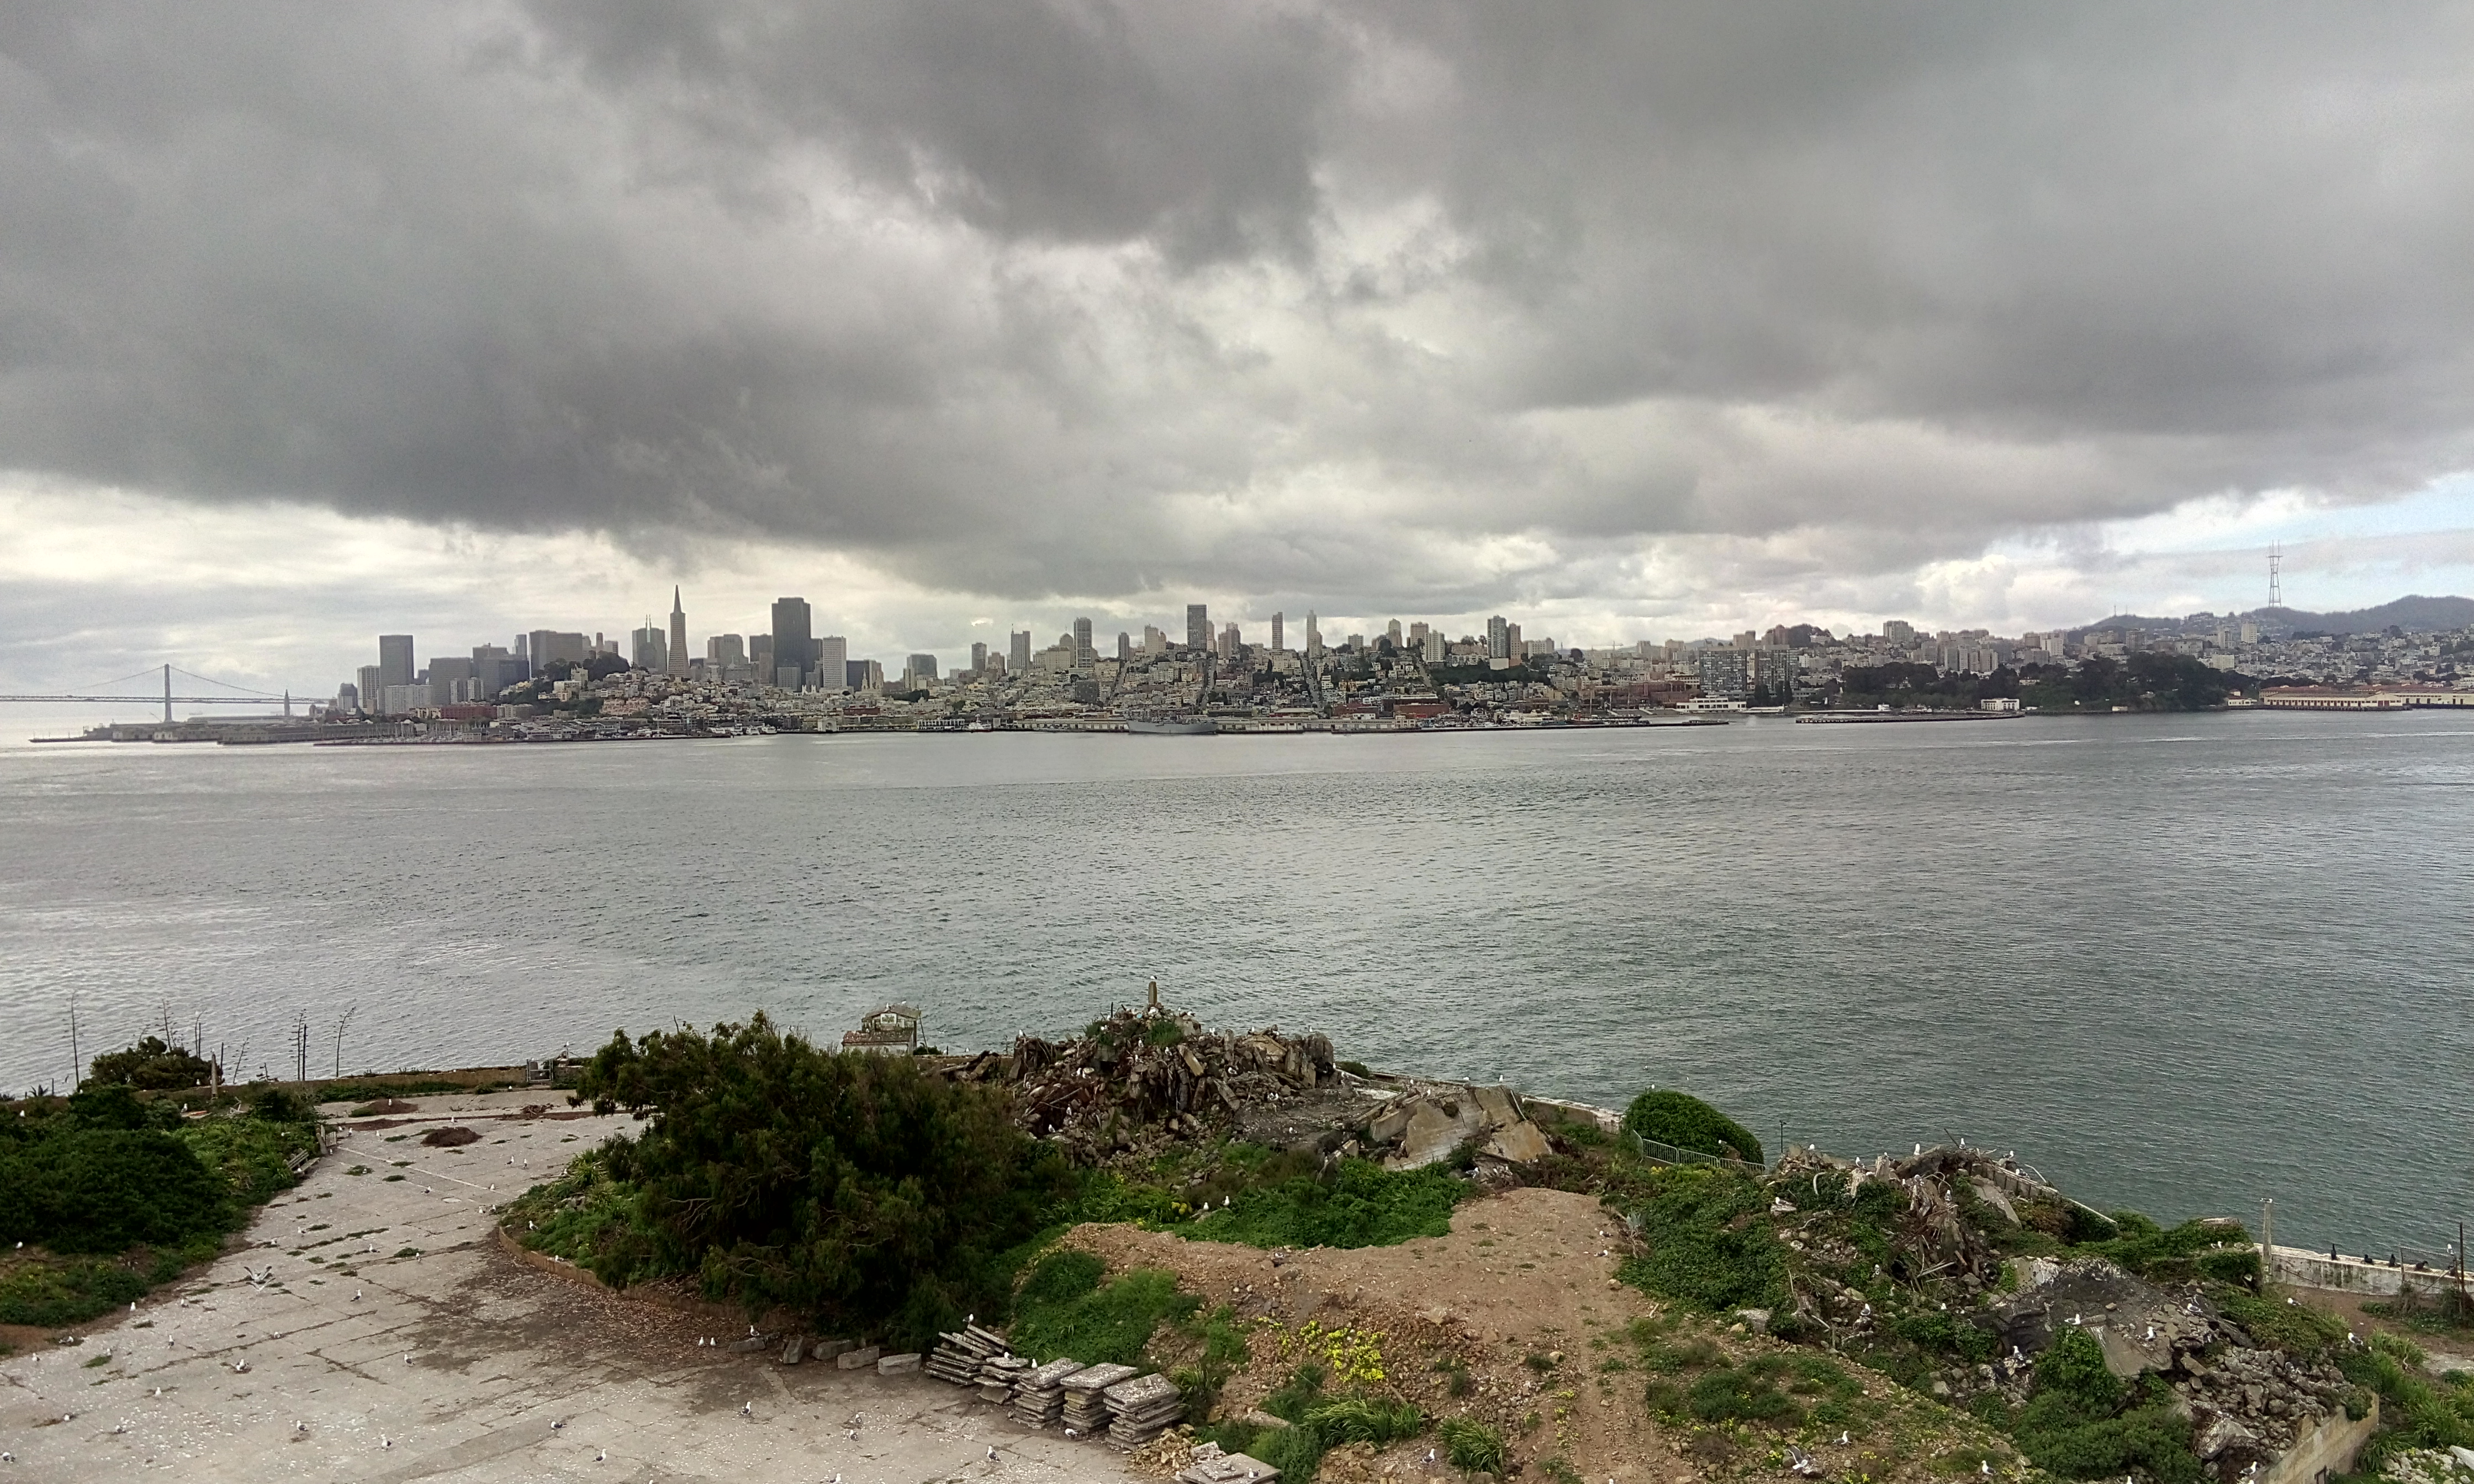
\includegraphics[width=\paperwidth,height=.5\paperheight]{21/image20160421_104822458.jpg};%
};
%\node[inner sep=0pt, yshift=.25\paperheight] at (current page.south) {%
%	\includegraphics[width=\paperwidth,height=.5\paperheight]{21/image20160420_193101911.jpg};%
%};
\end{tikzpicture}


\newpage
\thispagestyle{empty}
\begin{tikzpicture}[remember picture, overlay]
\node[inner sep=0pt, yshift=-.25\paperheight] at (current page.north) {%
	\includegraphics[width=\paperwidth,height=.5\paperheight]{21/image20160420_193101911.jpg};%
};
\end{tikzpicture}

\vspace*{.35\paperheight}

Im Anschluss suchten wir uns eine neue Unterkunft.
Die alte war zwar schön, aber leider auch schön Abseits von allem.
Im City Central Hostel wurden wir fündig.
Den restlichen Tag wollten wir in \FOREIGN{China Town} verbringen, aber da wir in die falsche Richtung gelaufen sind, wurde es eben \FOREIGN{Little Tokyo}.
Ewig konnten wir nicht umher streunen, denn für den Abend war der allwöchentliche \FOREIGN{Pub Crawl} angesagt.

Dort trafen wir in erster Linie andere Deutsche, Georg und Querin aus Mittenwald, einen Würzburger, der zum Thema Akkus promoviert und mir erklären konnte warum Tesla Autos mit größerer Reichweite bauen kann als die Anderen, und noch ein paar andere Gesichter.
Summa summarum waren wir in vier verschiedenen Pubs, eine Schwulenkneipe im Stadtteil \FOREIGN{The Castro} war auch dabei und hatten einen angenehmen Abend.
